%! TEX program = xelatex

\documentclass[Blue,dvipsnames]{beamer}

  \usepackage[utf8]{inputenc}
  \usepackage{utopia}            % font utopia imported
  \usepackage{amsmath}
  \usepackage{xeCJK}             % support Chinese
  \usepackage{calc}              % support command '\widthof'
  \usepackage{xcolor}
  \usepackage{enumitem} 
  \setlist[description]{%
  itemsep=5pt,                   % space between items
  font={\normalfont},            % set the label font
  font={\normalfont\sffamily\color{Blue}}, 
                                 % if colour is needed
  }

  \usetheme{Madrid}
  \usecolortheme{default}
  
 %v-v-v-v-v-v-v-v-v-v-v-v-v-v-v-v-v-v-v-v-v-v-v-v-v-v-v-v-v-v-v-v-
  %This block of code defines the information to appear in the
  %Title page
  \title[Postgraduate Recommendation] %optional
  {保研经验交流}
  
  \subtitle{(一个掺杂了各种主观认识的报告)}
  
  \author[Yang Li]
  {李洋\inst{1}}
  
  \institute[JLU] 
  {
    \inst{1}%
    Department of Physics\\
    Jilin University 
  }
  
  \date[JLU Physics 2018]
  {May 2018}
  
  %\logo{\includegraphics[height=1.5cm]{jlu.png}
  %End of title page configuration block
  %^-^-^-^-^-^-^-^-^-^-^-^-^-^-^-^-^-^-^-^-^-^-^-^-^-^-^-^-^-^-^-^-
  
  %v-v-v-v-v-v-v-v-v-v-v-v-v-v-v-v-v-v-v-v-v-v-v-v-v-v-v-v-v-v-v-v-
  %The next block of commands puts the table of contents at the 
  %beginning of each section and highlights the current section:
  
  \AtBeginSection[]
  {
    \begin{frame}
      \frametitle{Table of Contents}
      \tableofcontents[currentsection]
    \end{frame} 
  }
  %^-^-^-^-^-^-^-^-^-^-^-^-^-^-^-^-^-^-^-^-^-^-^-^-^-^-^-^-^-^-^-^-
  
  \begin{document}
  
    %v-v-v-v-v-v-v-v-v-v-v-v-v-v-v-v-v-v-v-v-v-v-v-v-v-v-v-v-v-v-v-v-
    %The next statement creates the title page.
    \frame{\titlepage}
    %^-^-^-^-^-^-^-^-^-^-^-^-^-^-^-^-^-^-^-^-^-^-^-^-^-^-^-^-^-^-^-^-
    
    %v-v-v-v-v-v-v-v-v-v-v-v-v-v-v-v-v-v-v-v-v-v-v-v-v-v-v-v-v-v-v-v-
    %This block of code is for the table of contents after
    %the title page
    \begin{frame}
    \frametitle{Table of Contents}
    \tableofcontents
    \end{frame}
    %^-^-^-^-^-^-^-^-^-^-^-^-^-^-^-^-^-^-^-^-^-^-^-^-^-^-^-^-^-^-^-^-
    
    \section{一些前置声明}  
    
    %v-v-v-v-v-v-v-v-v-v-v-v-v-v-v-v-v-v-v-v-v-v-v-v-v-v-v-v-v-v-v-v-
    %Changing visivility of the text
    \begin{frame}
    \frametitle{一些前置声明}
      首先声明本报告内容上的些许特性:

      \begin{description}[leftmargin=!,labelwidth=\widthof{\bfseries 不可重复}]
        \small
        \item[不可重复] 由于不同人情况不同, 本报告内容可能并不具备可重复性, 实际操作时请勿完全以此为准.
        \item[缺乏细节] 由于年代久远, 对一部分细节操作的记忆已相对模糊, 因此目前很难事无巨细地阐明这一过程.
        \item[存在引用] 本报告中的部分内容引用自13级学长, 遇此情况会特别说明. 
        \item[内容开源] 本报告内容完全开源, 您可以以任何非盈利目的分享此中信息. 通过访问作者\textbf{GitHub}相关项目网站, 获取此\textbf{Slides}源码:
        
        \url{https://github.com/epicODC/PublicPresentation}

      \end{description}
      \begin{block}{另外}
        报告过程中欢迎随时打断并提问.
      \end{block}
    \end{frame}
    %^-^-^-^-^-^-^-^-^-^-^-^-^-^-^-^-^-^-^-^-^-^-^-^-^-^-^-^-^-^-^-^-

    \section{呈递申请材料}  
    
    %v-v-v-v-v-v-v-v-v-v-v-v-v-v-v-v-v-v-v-v-v-v-v-v-v-v-v-v-v-v-v-v-
    %Changing visivility of the text
    \begin{frame}
    \frametitle{过程简述}

    一般准备阶段分以下几步:

    \begin{description}[leftmargin=!,labelwidth=\widthof{\bfseries 确定(导师及)学校}]
      \small
      \item[确定(导师及)学校] 确定心仪导师, 或者选定心仪学校及专业.
      \item[准备材料]        准备各种申报材料.(繁琐)
      \item[提交申请]        登录相关学校网站进行报名与文件提交. 
      \item[等待回复]        等待对方学校回复是否接受您参加面试.
    \end{description}

    \begin{block}{附注}
      对不同的学校, 所交材料种类和性质(纸质邮寄 或是 电子版 又或者是 两者混合)有所不同, 因此2,3两步实际操作时可能并没有区分度. 
    \end{block}
    \end{frame}
    %^-^-^-^-^-^-^-^-^-^-^-^-^-^-^-^-^-^-^-^-^-^-^-^-^-^-^-^-^-^-^-^-

    %v-v-v-v-v-v-v-v-v-v-v-v-v-v-v-v-v-v-v-v-v-v-v-v-v-v-v-v-v-v-v-v-
    %Changing visivility of the text
    \begin{frame}
      \frametitle{确定(导师及)学校}
        根据自己特长能力与兴趣选择心仪专业的老师. 如实在对自身潜力和未来发展没有任何认识和规划(只知道`我要做物理'), 又或者是对自己想进一步深造的专业现状没有任何概念, 则也可以学校名望为标准.

        \begin{block}{建议}
          可以找从事不同方向的学长或老师了解相关领域的内容和现状. 而后根据自身能力与兴趣进行理性的选择.
        \end{block}

        \begin{alertblock}{问题}
          目前国内部分高校缺少一个从事``本科生学科专业方向咨询,指导与规划''工作的老师. 显然,部分原因是此工作难度较高.
        \end{alertblock}

      \end{frame}
      %^-^-^-^-^-^-^-^-^-^-^-^-^-^-^-^-^-^-^-^-^-^-^-^-^-^-^-^-^-^-^-^-

      %v-v-v-v-v-v-v-v-v-v-v-v-v-v-v-v-v-v-v-v-v-v-v-v-v-v-v-v-v-v-v-v-
    %Changing visivility of the text
    \begin{frame}
      \frametitle{准备材料}
        通过浏览所选学校的相关网站, 注册并准备相关材料. 这些材料一般包括:

        \begin{description}[leftmargin=!,labelwidth=\widthof{\bfseries 个人简历}]
          \small
          \item[个人简历] 包括个人信息与自我陈述等模块, 不同学校要求不同.
          \item[相关证书] 各种获奖证书, 英语水平证明等.
          \item[成绩单]   通过逸夫楼或者经信楼成绩单打印机打印. 
          \item[推荐信]   不同老师(副教授或以上职称)签名的推荐信2-3封.
        \end{description}

        \begin{alertblock}{问题}
          一般申报的数所学校要求呈递的材料种类和属性均有所差异, 有些学校甚至有预报名与正式报名之分. 因此, 如处理不当, 极有可能一连几星期都奔波在打印店, 教务处, 推荐信老师办公室与鼎新楼之间.
        \end{alertblock}

        \begin{block}{一种解决方案}
          建议建立一套个人信息电子档案系统.
        \end{block}
      \end{frame} 
      %^-^-^-^-^-^-^-^-^-^-^-^-^-^-^-^-^-^-^-^-^-^-^-^-^-^-^-^-^-^-^-^-

      %v-v-v-v-v-v-v-v-v-v-v-v-v-v-v-v-v-v-v-v-v-v-v-v-v-v-v-v-v-v-v-v-
    %Changing visivility of the text
    \begin{frame}
      \frametitle{准备材料}
        建立个人信息电子档案系统(该方法引自某13级学长):
        \begin{figure} 
          \fbox{\centering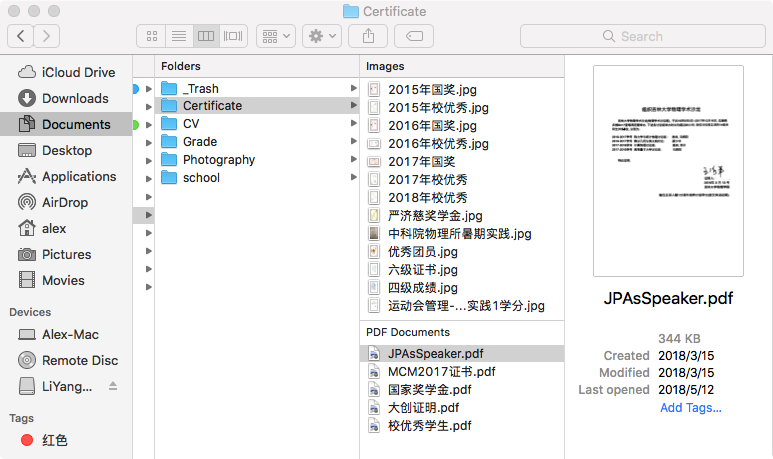
\includegraphics[width=4in]{figure/PersonalInfo}}
          \caption{个人信息电子档案系统}
        \end{figure} 
      \end{frame} 
      %^-^-^-^-^-^-^-^-^-^-^-^-^-^-^-^-^-^-^-^-^-^-^-^-^-^-^-^-^-^-^-^-

      %v-v-v-v-v-v-v-v-v-v-v-v-v-v-v-v-v-v-v-v-v-v-v-v-v-v-v-v-v-v-v-v-
      %Changing visivility of the text
      \begin{frame}
      \frametitle{提交申请}
        根据不同学校提交申请的要求, 纸质邮寄或者网上提交您准备完善的个人申请材料.
        \begin{block}{附注}
          提交过程可能并非一次性完成, 请实时关注您的邮箱以及官方网站动态.
        \end{block}
        \begin{block}{Remark}
         如果此时已经建立了一套自己的档案系统, 您会发现当前阶段您会相对从容.
        \end{block}
      \end{frame}
      %^-^-^-^-^-^-^-^-^-^-^-^-^-^-^-^-^-^-^-^-^-^-^-^-^-^-^-^-^-^-^-^-

      %v-v-v-v-v-v-v-v-v-v-v-v-v-v-v-v-v-v-v-v-v-v-v-v-v-v-v-v-v-v-v-v-
      %Changing visivility of the text
      \begin{frame}
      \frametitle{等待回复}
      确定正确提交全部申请材料后, 请耐心等待初审结果. 一般官方网站会在指定时间放出初审通过名单, 并以邮件(或电话)的方式提醒您可以参加面试.
      \begin{block}{一条合理的建议}
        申请同所学校的同学可以建一个交流群, 方便互相提醒.  
      \end{block}
      \end{frame}
      %^-^-^-^-^-^-^-^-^-^-^-^-^-^-^-^-^-^-^-^-^-^-^-^-^-^-^-^-^-^-^-^-

    \section{参加(笔试与)面试} 
    
    %v-v-v-v-v-v-v-v-v-v-v-v-v-v-v-v-v-v-v-v-v-v-v-v-v-v-v-v-v-v-v-v-
    %Changing visivility of the text
    \begin{frame}
    \frametitle{简单介绍}
    关于夏令营:
    \begin{enumerate}[label=--]
      \item 如果您通过了初审, 那么您将有机会参加有关学校或研究所的的夏令营. 夏令营一般在当年暑期或接近暑期时举行, 为期数日, 由相关院校提供食宿.
      \item 学院相关任课老师会特意调整(提前)期末考试时间, 以防止与保研夏令营冲突.
      \item 但不同学校或研究所之间夏令营可能冲突, 请理性取舍.
      \item 不同学校及同一学校不同院系的考核手段(笔试,面试)可能会有所不同. 具体考核方式, 请参考具体通知.
    \end{enumerate}
    \begin{block}{两条合理的建议}
      \small
      事前合理规划参加夏令营期间的行程, 以及适当调研相关路线或许是十分有帮助的.(否则可能一直宅在酒店里无所事事, 又或者是手忙脚乱地前往面试地点.)另外, 将电子档案随身携带将会是十分明智的选择.
    \end{block}
    \end{frame}
    %^-^-^-^-^-^-^-^-^-^-^-^-^-^-^-^-^-^-^-^-^-^-^-^-^-^-^-^-^-^-^-^-

    %v-v-v-v-v-v-v-v-v-v-v-v-v-v-v-v-v-v-v-v-v-v-v-v-v-v-v-v-v-v-v-v-
    %Changing visivility of the text
    \begin{frame}
      \frametitle{参加(笔试与)面试}
      \small
      \begin{block}{一些主观看法 1}
        避免对面试过于``敏感'', 面试时的你应该和平时的你有相同的行为和表现.
      \end{block}
      \begin{alertblock}{一些主观看法 2}
        任何面试前突击的想法都不切实际, 任何在面试中刻意装模作样的尝试都将被一眼戳穿.
      \end{alertblock}
      \begin{block}{一些主观看法 3}
        面试只是个人平时表现和学识的自然流露. 讲到底, 任何焦虑不安情绪的根源, 都是意识到自己正在试图获取超出自身能力范围之外的成果.
      \end{block}
      \begin{block}{一些主观看法 4}
        以上几条同样适用于笔试, 唯一不同的是, 笔试前最好适当做点题热热身.
      \end{block}

      \end{frame}
      %^-^-^-^-^-^-^-^-^-^-^-^-^-^-^-^-^-^-^-^-^-^-^-^-^-^-^-^-^-^-^-^-

      %v-v-v-v-v-v-v-v-v-v-v-v-v-v-v-v-v-v-v-v-v-v-v-v-v-v-v-v-v-v-v-v-
      %Changing visivility of the text
      \begin{frame}
      \frametitle{参加(笔试与)面试}
      \begin{block}{一些主观看法 5}
        由于不清楚自己的实力到底在竞争者中处于什么水平, 面试刚开始可能会有点紧张. 但是和面试老师聊开之后就会轻松很多.
      \end{block}

      \begin{block}{一些主观看法 6}
        经历过面试之后再想一想, 也无非就是和未来的任课老师或者老板或者学长提前聊聊天, 认识一下.
      \end{block}

      \begin{block}{一些主观看法\  总结}
        顺其自然, 有实力者自得之.
      \end{block}
      \end{frame}
      %^-^-^-^-^-^-^-^-^-^-^-^-^-^-^-^-^-^-^-^-^-^-^-^-^-^-^-^-^-^-^-^-

      %v-v-v-v-v-v-v-v-v-v-v-v-v-v-v-v-v-v-v-v-v-v-v-v-v-v-v-v-v-v-v-v-
      %Changing visivility of the text
      \begin{frame}
        \frametitle{参加(笔试与)面试}
        如果您通过面试, 相关负责人会以邮件(或电话)的方式通知您以通过面试. 此时或许需要您在一定期限内做出决定, 是否最终确定接受此offer, 并同意跟随所选导师进行日后的学习与科研. 
        
        \begin{block}{另外}
          其他院校的夏令营可能会在该期限以外举行, 届时请理性选择.
        \end{block}
        
        \end{frame}
        %^-^-^-^-^-^-^-^-^-^-^-^-^-^-^-^-^-^-^-^-^-^-^-^-^-^-^-^-^-^-^-^-

    \section{确认预录取信息}  
    
    %v-v-v-v-v-v-v-v-v-v-v-v-v-v-v-v-v-v-v-v-v-v-v-v-v-v-v-v-v-v-v-v-
    %Changing visivility of the text
    \begin{frame}
    \frametitle{确认预录取信息}
    如果您顺利通过夏令营保研面试, 下一学期再次返校后注意以下事项:
    \begin{description}[leftmargin=!,labelwidth=\widthof{\bfseries 录取信息确认}]
      \small
      \item[保研资格] 请再此确认您是否真的有保研资格. (这一信息应在填报申请材料时确认过一次)
      \item[保研条件] 虽然通过夏令营您已经基本可以保研, 但一般还需要在接下来的一年中达成一定的条件.(具体可参考相关院校官网的说明)
      \item[正式申请] 开学一段时间之后, 您需要在学信网上进行教育部认可的正式的研究生报名. 该操作一般并不像通知的那样时间宽松. 如收到类似通知, 请立刻前往报名. 具体操作参考相关邮件通知和学院内部的通知.
      \item[毕业论文] 基本确认保研后, 部分导师会提供进组实习及写毕业论文的机会. 请与相关老师或学长确认, 组内是否有此惯例. 
    \end{description} 

    {
      \setbeamercolor{block title}{bg=orange, fg=white}
      \begin{block}{\small{一些个人看法}}
        通过面试是一段更加努力的日子的开始, 为此需要做足准备. 同时, 任何努力都不会白费. 
      \end{block}
    }
    \end{frame}
    %^-^-^-^-^-^-^-^-^-^-^-^-^-^-^-^-^-^-^-^-^-^-^-^-^-^-^-^-^-^-^-^-
    %v-v-v-v-v-v-v-v-v-v-v-v-v-v-v-v-v-v-v-v-v-v-v-v-v-v-v-v-v-v-v-v-
    %Changing visivility of the text
    \begin{frame}
      \frametitle{确认预录取信息}
      \begin{block}{一条合理的建议}
        最后是一条个人建议. 您可能已经在夏令营中体会到了, 目前学院所开设专业课程进程缓慢而基础. 鉴于您目前已经基本无虑, 可以立刻开始着手学习研究生专业知识以及进组实习. 
      \end{block}
      {\small\textcolor{gray}{如果您恰好个人能力较强, 从而不存在此问题, 那这真是一件令人欣慰的事情.}}
    \end{frame}

    \section{总结}  

    %v-v-v-v-v-v-v-v-v-v-v-v-v-v-v-v-v-v-v-v-v-v-v-v-v-v-v-v-v-v-v-v-
    %Changing visivility of the text
    \begin{frame}
      \frametitle{总结}
      总而言之:
        \begin{enumerate}[label=--]
          \item 实际报考前, 请确定自己心仪的专业, 老师或学校.
          \item 申请材料准备与寄送过程十分繁琐, 建立一个电子档案或许是十分有帮助的.
          \item 笔试与面试过程中请保持淡定, 有实力者自得之.
          \item 通过面试后还需要正式报名, 请勿眼高手低.
        \end{enumerate}
        {
          \setbeamercolor{block title}{bg=orange, fg=white}
          \begin{block}{\small{最后}}
            祝学弟学妹们拿到心仪的offer.
          \end{block}
          }

      \end{frame}
      %^-^-^-^-^-^-^-^-^-^-^-^-^-^-^-^-^-^-^-^-^-^-^-^-^-^-^-^-^-^-^-^-

      %v-v-v-v-v-v-v-v-v-v-v-v-v-v-v-v-v-v-v-v-v-v-v-v-v-v-v-v-v-v-v-v-
    %Changing visivility of the text
    \begin{frame}
      \frametitle{更多信息}
      \begin{block}{开源声明}
        本报告内容完全开源, 您可以以任何非盈利目的分享此中信息. 访问\textbf{GitHub}相关项目网站, 获取此\textbf{Slides}源码及更多信息:
        
        \Large\url{https://github.com/epicODC/PublicPresentation}
      \end{block}

    \end{frame}
      %^-^-^-^-^-^-^-^-^-^-^-^-^-^-^-^-^-^-^-^-^-^-^-^-^-^-^-^-^-^-^-^-
  \end{document}